%%%%
% Consiglio la visione dei seguenti tutorial:
% - https://www.youtube.com/watch?v=ihxSUsJB_14
% - https://www.youtube.com/watch?v=XTFWaV55uDo
%%%%
\documentclass[12pt,a4paper,openright,twoside]{book}
\usepackage[utf8]{inputenc}
\usepackage{float}
\usepackage{hyperref}

\newcommand{\thesislang}{italian} % decommentare in caso di tesi in italiano
%\newcommand{\thesislang}{english} % commentare in caso di tesi in italiano
\usepackage{thesis-style}

\begin{document}
	
\frontmatter

% ! TeX root = thesis-main.tex
\title{Title}
\author{Candidate Name Here}
\date{\today}

\begin{titlepage}
	\begin{center}
		% \vspace*{0.2cm}
		
		\large
		\textbf{ALMA MATER STUDIORUM -- UNIVERSITÀ DI BOLOGNA \\ CAMPUS DI CESENA}
		\\
		\noindent\hrulefill
		\vspace{0.4cm}
		
		\Large
		Scuola di Ingegneria e Architettura \\
		Corso di Laurea Magistrale in Ingegneria e Scienze Informatiche
		
		\Huge
		\vspace{4cm}
		\textbf{Assignment \#02}
		
		\large
		\vspace{1cm}
		Elaborato in 
		\\
		\textsc{Programmazione concorrente e distribuita}
		
		\vspace{5.5cm}
		\begin{minipage}[t]{0.64\textwidth}
			\begin{flushleft}
			\end{flushleft}
		\end{minipage}
		\begin{minipage}[t]{0.34\textwidth}
			\begin{flushright}
				\textit{Studenti} 
				\\ 
				\textbf{Eddie Barzi}
				\\ 
				\textbf{Filippo Vissani}
			\end{flushright}
		\end{minipage}\\
		
		\vfill
		\noindent\hrulefill
		\vspace{0.3cm}
		\Large

		Anno Accademico 2021-2022
	\end{center}
\end{titlepage}
\restoregeometry


%----------------------------------------------------------------------------------------
\tableofcontents   
%\listoffigures     % (optional) comment if empty
%\lstlistoflistings % (optional) comment if empty
%----------------------------------------------------------------------------------------

\mainmatter

%----------------------------------------------------------------------------------------
\chapter{\introductionname}
\label{chap:introduction}
%----------------------------------------------------------------------------------------
\section{Descrizione e Obiettivi}
\subsection{Task Frameworks}
Viene fornito il codice di un programma che simula il movimento di $N$ corpi su un piano bidimensionale,
soggetti a due tipi di forze:
\begin{itemize}
	\item una forza repulsiva, per cui ogni corpo $b_{i}$ esercita su ogni altro corpo $b_{j}$ una forza in modulo pari a:
	\begin{center}
		$ F_{ij} = \frac{k_{rep} \times m_{i}}{d^2_{ij}} $
	\end{center}
	Dove $m_{i}$ è la massa del corpo $b_{i}$, $k_{rep}$ è una costante data, $d_{ij}$ è la distanza fra i due corpi.
	La direzione della forza è data dal versore $(b_{i} - b_{j})$, ovvero respingente per il corpo $b_{j}$.
	\item Una forza di attrito, per cui su ogni corpo $b_{i}$ che si muove a una velocità $v_{i}$ è esercitata una forza:
	\begin{center}
		$ FR_{i} = - k_{fri} \times v_{i} $
	\end{center}
	Che si oppone al moto, quindi in direzione opposta alla sua velocità, dove $k_{fri}$ è una costante data.
\end{itemize}
Il programma è sequenziale, non strutturato. 
L'algoritmo \ref{lst:lst1} definisce il comportamento del simulatore in pseudo codice.
\newpage
\begin{lstlisting}[label=lst:lst1,caption=Pseudocodice del programma sequenziale]
/* virtual time */
vt = 0;
/* time increment at each iteration */     
dt  = 0.01;

loop:
	for each body b[i]:
		compute total force exerted by other bodies b[j] and friction;
		compute the instant acceleration, given the total force and mass;
		update body velocity, given the acceleration and the virtual time elapsed dt;
	update bodies positions, given the velocity and virtual time elapsed dt;
	check boundary collisions;
	vt = vt + dt;   
	display current stage;

\end{lstlisting}

Alcuni aspetti rilevanti in merito al comportamento del programma e alla natura del problema:
\begin{itemize}
	\item Il calcolo delle forze al tempo $t$ avviene considerando coerentemente le posizioni dei corpi al tempo $t$. 
	\item L'aggiornamento delle posizioni può avvenire solo dopo che tutte le forze sono state calcolate (e le velocità aggiornate).
	\item Il controllo della collisione con i confini del mondo per un corpo $b_{i}$ può comportare il cambiamento della velocità e posizione del corpo.
	\item Nel programma, la visualizzazione dello stato corrente della simulazione o frame (via GUI) avviene in modo sincrono, per cui la successiva iterazione avviene solo dopo aver visualizzato lo stato della precedente.
\end{itemize}

Si vuole realizzare una versione concorrente della simulazione senza GUI, considerando un insieme iniziale $N$ di corpi
- e calcolando l'evoluzione temporale per un certo numero di passi $Nsteps$ -
con $Nsteps$ fissato come parametro. Posizione e velocità iniziali possono essere definite in modo casuale.
L'obiettivo è:
\begin{itemize}
	\item Massimizzare le performance, sfruttando tutte le capacità di calcolo del generico
	sistema di elaborazione su cui è mandato in esecuzione il programma.
	\item Organizzare il programma in modo modulare, estendibile.
\end{itemize}

Inoltre si vogliono analizzare le performance del programma considerando valori di $N$ pari a 100, 1000, 5000, con $Nsteps$ pari a 1000, 10000, 50000,
calcolando lo speedup, e valutando il suo comportamento usando sia il numero ottimale teorico di thread,
sia considerando prove diverse con un numero variabile di threads per verificarne la scalabilità.

Infine si vuole verificare la correttezza del programma usando Java Path Finder, considerando la parte più significativa in merito, opportunamente semplificata.
Estendere la simulazione includendo una GUI con pulsanti start/stop per lanciare/fermare la simulazione e visualizzare l'andamento,
includendo informazioni circa il tempo virtuale.
La GUI si presuppone visualizzi stati consistenti della simulazione (ma non necessariamente tutti gli stati).

\subsection{Event-Driven Asynchronous Programming}
JavaParser (\href{http://javaparser.org/}{http://javaparser.org/}) è una libreria open-source che fornisce funzionalità per fare il parsing e l'analisi di codice sorgente Java, costruendo l'AST e permettendo di navigare l'albero  con il pattern Visitor. La libreria lavora a livello di singolo file.

Si vuole creare una libreria con API asincrona (basata su event-loop) che permetta di fornire un insieme di funzionalità minimale di analisi di un progetto Java, potendo sfruttare nella sua implementazione JavaParser. 
Le funzionalità che la libreria dovrà fornire sono:
\begin{itemize}
    \item \texttt{interfaceReport}: metodo asincrono per ottenere il report di una specifica interfaccia. Il report di una interfaccia contiene il nome, il nome completo (comprende i genitori) e info su essenziali sui metodi (nome)
    \item \texttt{classReport}: metodo asincrono per ottenere il report di una specifica classe. Il report di una classe contiene il nome, il nome completo (comprende i genitori), info essenziali sui metodi (nome, visibilità, posizione nel file: inizio linea, fine linea), info essenziali sui campi (nome, tipo) e se è una main class
    \item \texttt{packageReport}: metodo asincrono per costruire il report di uno specifico package. Il report di un package contiene nome completo del package e informazioni (report) relativamente alle classi e interfacce che appartengono al package
    \item \texttt{projectReport}: metodo asincrono per costruire il report di un progetto intero. Il report di un progetto contiene informazioni (report) circa i package che appartengono al progetto e l'indicazione di quale sia la main class
    \item \texttt{analyzeProject}: metodo asincrono per poter effettuare un'analisi incrementale di un progetto, generando eventi per gli elementi man mano incontrati (campi, metodi, classi, interfacce, package)

\end{itemize}


Data la libreria, costruire una semplice applicazione con GUI che consenta di:
\begin{itemize}
    \item selezionare il project folder
    \item far partire analisi e poterla eventualmente interrompere, in modo responsivo
    \item visualizzare man mano gli elementi trovati, in forma opportuna
\end{itemize}

Adottare un approccio basato su framework di programmazione ad eventi ad event-loop. Esempio di riferimento visto nel corso: Vert.x, in Java o nel linguaggio che si preferisce.

\subsection{Reactive Programming}
Realizzare una soluzione al problema descritto precedentemente, basata su programmazione reattiva.
In particolare, si richiede di:
\begin{itemize}
    \item ripensare alla libreria in modo che abbia anche l'interfaccia in linea con l'approccio paradigmatico caratterizzante la programmazione reattiva.
    \item  sviluppare la semplice applicazione in modo che usi la libreria.
\end{itemize}
Adottare un approccio basato su estensioni RX.
%----------------------------------------------------------------------------------------
\chapter{Analisi del Problema}
\label{chap:Analisi del Problema}
%----------------------------------------------------------------------------------------
\section{Task Frameworks}
Portando il programma da sequenziale a parallelo devono essere considerati i seguenti aspetti:
\begin{itemize}
	\item Più flussi di esecuzione accedono in modo concorrente alla stessa lista di corpi.
	Quindi è necessario che i flussi siano sincronizzati (evitando deadlock, race contition, ecc...).
	\item La sincronizzazione deve avvenire in modo efficiente; bisogna sfruttare al massimo il tempo per
	la computazione evitando attese non necessarie.
	\item A ogni iterazione, dati due flussi di esecuzione $f_{i}$ e $f_{j}$, i quali eseguono computazioni su due corpi $c_{k}$ e $c_{w}$ rispettivamente (con $i \neq j$ e $k \neq w$),
	$f_{i}$ non deve aggiornare la posizione di $c_{k}$ prima che $f_{j}$ abbia terminato di calcolare la forza esercitata su $c_{w}$.
	\item La rappresentazione della simulazione deve rimanere
	consistente, i flussi devono essere sempre sincronizzati sulla
	stessa iterazione.
	\item È fondamentale che il numero di flussi di esecuzione venga scelto sulla base dei processori disponibili sulla macchina, ovvero
	rispettando la formula $N_{cpu} + 1$, per minimizzare il tempo di esecuzione.
	\item È buona pratica separare i componenti che riguardano la concorrenza dagli aspetti di logica e di grafica,
	così da rendere il sistema modulare ed estendibile.
	\item Gli eventi relativi alla pressione dei pulsanti
	devono essere gestiti atomicamente, dato che si occupano di
	avviare e fermare i flussi di esecuzione.
	\item Al termine della simulazione, sia nel caso in cui sia stato raggiunto
	il numero massimo di iterazioni, che nel caso in cui sia stato premuto il
	pulsante Stop, tutti i flussi di esecuzione devono terminare correttamente.
\end{itemize}

\section{Event-Driven Asynchronous Programming e Reactive Programming}
Per quanto riguarda la progettazione e lo sviluppo della libreria asincrona e dell'applicazione grafica, sia che si tratti di programmazione ad eventi che di programmazione reattiva, bisogna considerare i seguenti aspetti:

Nel metodo \texttt{packageReport} il parsing delle classi e delle interfacce deve essere parallelizzato a livello di file, in altre parole la computazione dei file all'interno di un package non deve essere demandata a un singolo flusso di esecuzione.

Allo stesso modo, il metodo \texttt{projectReport} deve creare i report dei vari package sfruttando più flussi di esecuzione.
Grazie a questa tecnica il tempo di esecuzione viene minimizzato e vengono sfruttati tutti i processori presenti sulla macchina; l'unica limitazione è data dall'accesso concorrente al filesystem, che potrebbe rallentare la computazione.

Nel metodo \texttt{analyzeProject} sorge la necessità di utilizzare un canale condiviso fra più flussi di esecuzione per l'invio e la ricezione di messaggi, quindi l'ordine di invio e di ricezione dei report non è deterministico.
Per visualizzare correttamente la gerarchia degli elementi del progetto è necessario implementare un algoritmo che riordini gli elementi che vengono ricevuti sul canale.
%----------------------------------------------------------------------------------------
\chapter{Descrizione dell'Architettura Proposta}
\label{chap:Descrizione dell'Architettura Proposta}
%----------------------------------------------------------------------------------------
Per la realizzazione delle diverse parti dell'assignment si è scelto di adottare tecnologie differenti.
Per la versione del primo assignment orientata a task si è scelto di utilizzare Java, dato che le modifiche da apportare erano esigue.
Per il secondo e il terzo punto invece, a scopo didattico, si è scelto di impiegare Scala.

\section{Task Frameworks}
In fase di progettazione, per separare al meglio gli aspetti di logica e grafica da quelli di concorrenza, si è scelto di impiegare il pattern architetturale \textit{Model-View-Controller} (Figura \ref{fig:tfmvc}).
Nel \textit{Model} viene gestito l'aggiornamento della posizione dei corpi a ogni iterazione. In particolare viene fornita 
un'interfaccia di programmazione con i seguenti metodi (vengono riportati solo i più significativi):
\begin{itemize}
	\item \texttt{checkAndSolveBoundaryCollisionOnBodiesRange(range)}: 
	utilizzato per risolvere le collisioni di un intervallo di corpi con i bordi della simulazione.
	\item \texttt{updatePositionOnBodiesRange(range)}:
	utilizzato per aggiornare la posizione di un intervallo di corpi.
	\item \texttt{computeAccelerationOnBodiesRange(range)}:
	utilizzato per calcolare l'accelerazione di un intervallo di corpi.
	\item \texttt{updateSpeedOnBodiesRange(range, acceleration)}:
	utilizzato per aggiornare la velocità di un intervallo di corpi.
\end{itemize}
Nei metodi appena descritti viene specificato sempre l'intervallo di corpi per permettere ai task di agire su porzioni differenti della lista senza generare race condition.

Gli aspetti di concorrenza vengono gestiti completamente nel \textit{Controller},
descritto più dettagliatamente in Figura \ref{fig:tfc}.
La classe \texttt{SimulationManager}, che implementa l'interfaccia \texttt{Runnable}, crea due tipi di task per ogni range di corpi:
\begin{itemize}
    \item \texttt{UpdateSpeedTask:} si occupa di calcolare l'accelerazione su un intervallo di corpi e poi aggiornarne la velocità.
    \item \texttt{UpdatePositionTask:} si occupa di aggiornare la posizione di un intervallo di corpi e controllare eventuali collisioni.
\end{itemize}
Entrambi i task implementano \texttt{Callable} e restituiscono il risultato di un \texttt{Future} al loro completamento. In questo modo viene gestita la concorrenza, eseguendo prima tutti i task di tipo \texttt{UpdateSpeedTask} e poi tutti i task di tipo \texttt{UpdatePositionTask}.

Nel \textit{Controller} è presente il metodo \texttt{stopSimulation}, il quale imposta un flag per interrompere la simulazione all'iterazione corrente.
Inoltre il \textit{Controller} si occupa di aggiornare la \textit{View} ad ogni iterazione.

La \textit{View} (Figura \ref{fig:tfgui}) oltre a rappresentare lo stato corrente della simulazione, 
riporta il tempo virtuale e l'iterazione correnti.
L'interfaccia grafica dispone anche di due pulsanti, utilizzati per avviare e fermare la simulazione.
\begin{figure}[H]
	\centering
	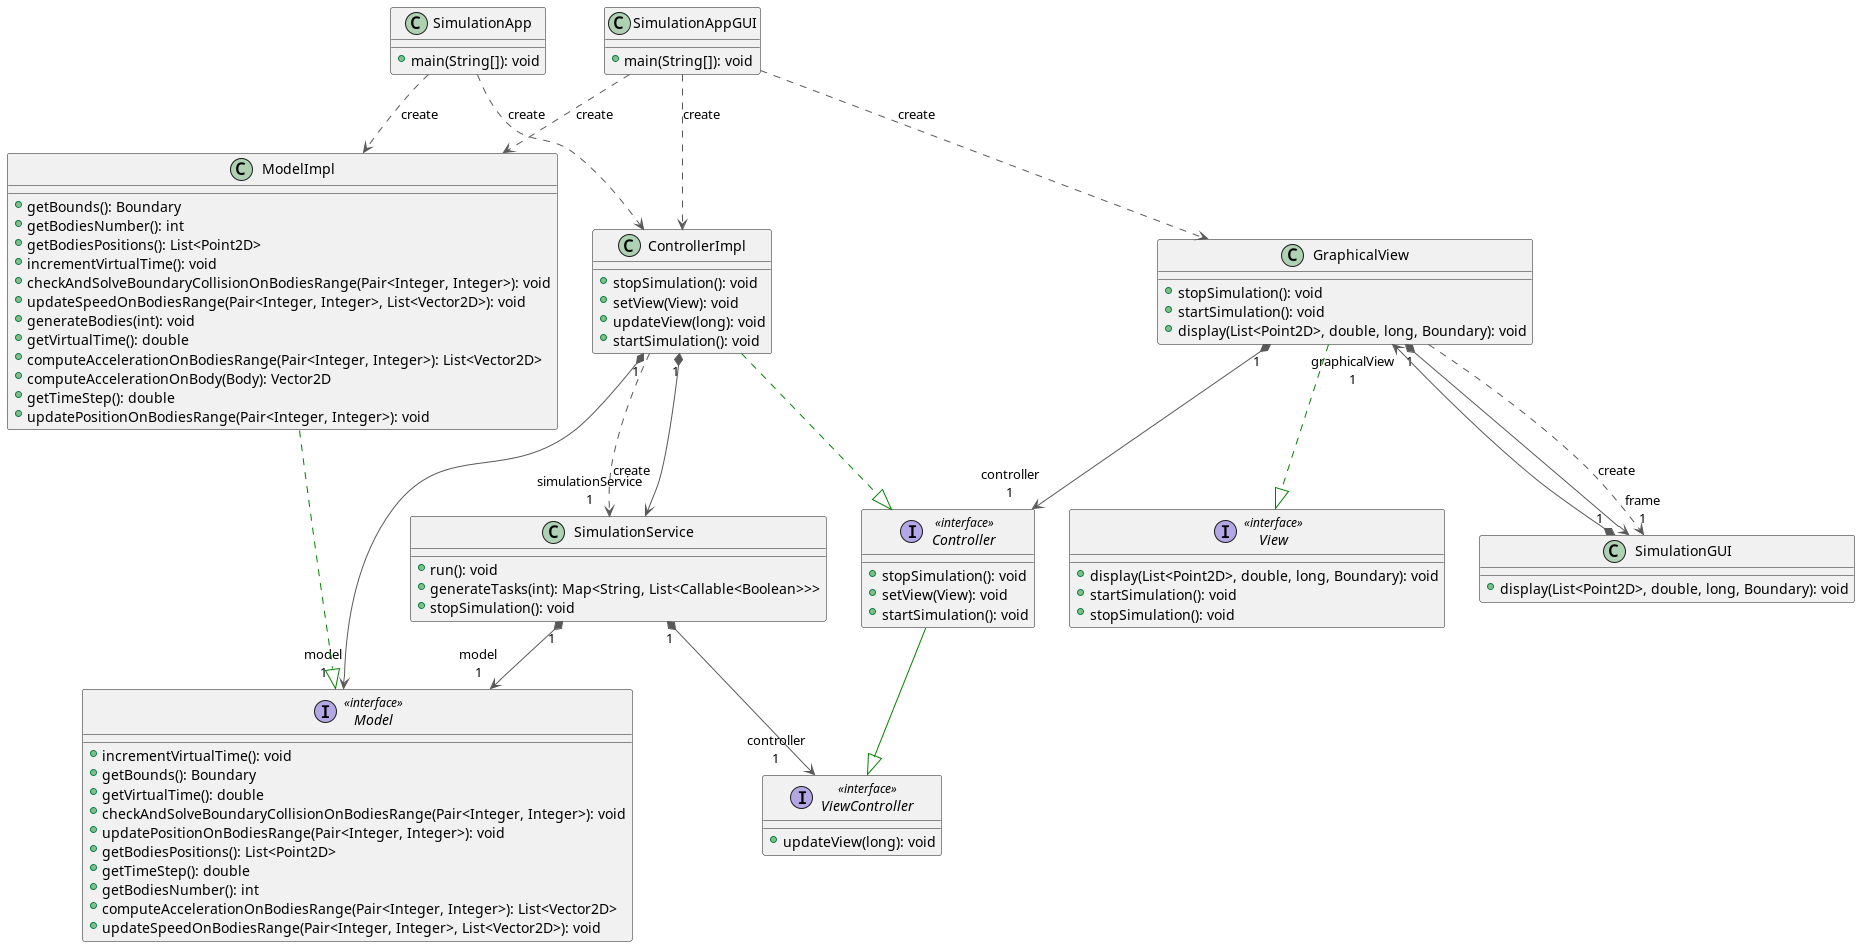
\includegraphics[angle=90, height=\textheight]{figures/TFMVC-0.png}
	\caption{Task Frameworks: Model-View-Controller.}
	\label{fig:tfmvc}
\end{figure}
\begin{figure}[H]
	\centering
    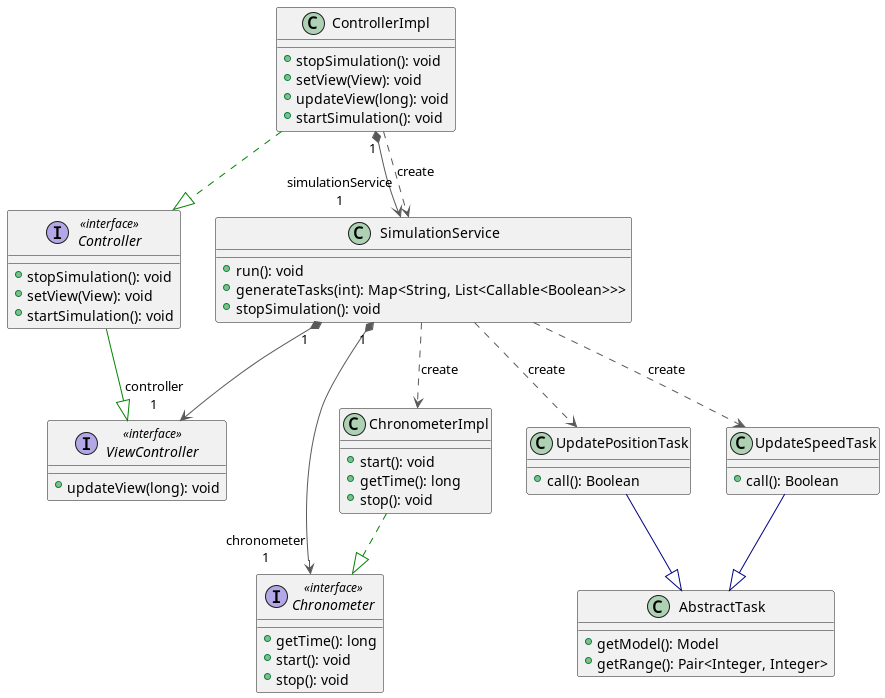
\includegraphics[width=\textwidth]{figures/TFController-0.png}
	\caption{Task Frameworks: Controller.}
	\label{fig:tfc}
\end{figure}
\begin{figure}[H]
	\centering
	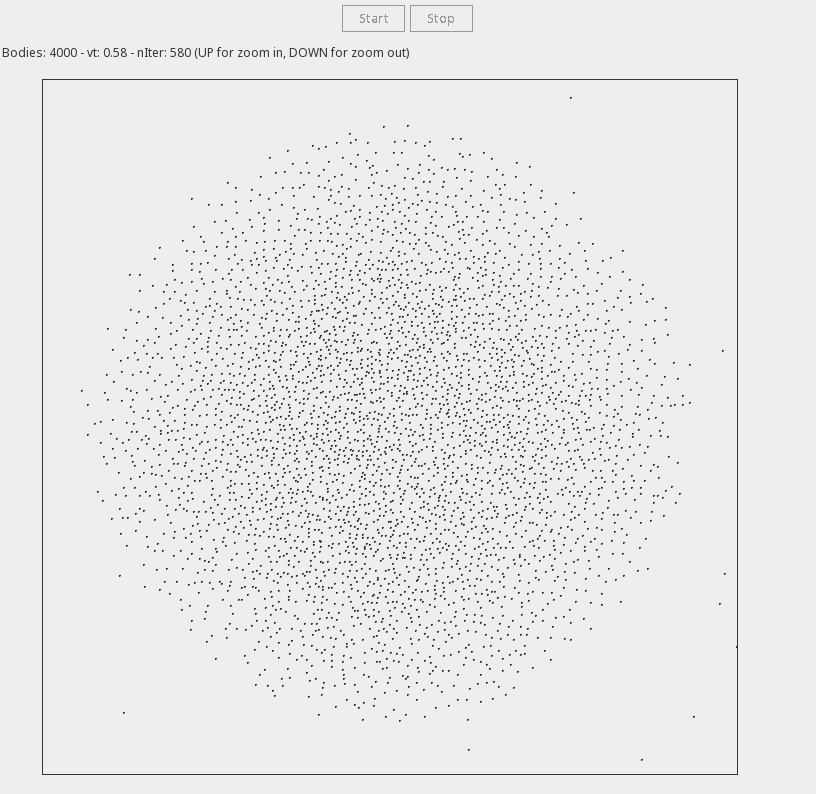
\includegraphics[width=\linewidth]{figures/simulation.png}
	\caption{Task Frameworks: Interfaccia grafica}
	\label{fig:tfgui}
\end{figure}

\section{Event Driven Asynchronous Programming e Reactive Programming}
Nell'implementazione \textit{Event Driven} della libreria Project Analyzer (Diagramma delle classi rappresentato in Figura \ref{fig:edappa}) si è scelto di utilizzare il framework \textit{Vert.x}.
Project Analyzer è quindi stata concepita per essere sfruttata all'interno di un \textit{Verticle}.
I metodi della libreria fanno uso della funzionalità \texttt{Vertx.executeBlocking}, che permette di eseguire computazioni in modo asincrono sfruttando i \textit{Future} e le \textit{Promise}.
Per eseguire il parsing dei file Java è stata impiegata la libreria JavaParser, che adotta il pattern \textit{Visitor}.
Più nel dettaglio, sono stati creati due \textit{Collector} che estendono \texttt{VoidVisitorAdapter}:
\begin{itemize}
    \item \texttt{FutureCollector}: si occupa di eseguire semplicemente la visita di campi e metodi e di generare il report in modo incrementale
    \item \texttt{EventBusCollector}: come \texttt{FutureCollector}, ma allo stesso tempo pubblica gli elementi trovati sull'\textit{Event Bus} di \textit{Vert.x}
\end{itemize}

Per quanto riguarda l'interfaccia grafica, si è scelto anche in questo caso di adottare il pattern \textit{Model-View-Controller} (Figura \ref{fig:edapmvc}).
Il Controller dispone di un \textit{Verticle} che si occupa di utilizzare la libreria Project Analyzer.
In particolare, il \textit{Verticle} sfrutta determinati \textit{Topic} per ricevere correttamente i messaggi provenienti dall'\textit{Event Bus}.
I messaggi codificati in Json, una volta ricevuti, vengono convertiti nuovamente a oggetti e vengono passati al \texttt{TreeGenerator} (Figura \ref{fig:edapta}), che si occupa di ricreare correttamente l'albero della gerarchia.
L'albero riordinato viene infine passato alla View, che lo mostra all'utente.

L'interfaccia grafica (Figura \ref{fig:edapgui}) permette all'utente di scegliere il progetto Java da analizzare e far partire e fermare l'analisi.

Le implementazioni \textit{Reactive} di Project Analyzer e dell'applicazione hanno un comportamento simile alle implementazioni \textit{Event Driven} (il diagramma delle classi non viene riportato perché le variazioni sono minime).
In Project Analyzer le funzionalità che sfruttavano \texttt{Vertx.executeBlocking} ora impiegano i \texttt{Flowable} di \textit{RXJava}.
L'\textit{Event Bus} di \textit{Vertx} è stato sostituito con \texttt{PublishSubject} ed è stata sfruttata una \texttt{Map} per implementare una soluzione simile ai \textit{Topic} dell'\textit{Event Bus} di \textit{Vert.x}.

\begin{figure}
	\centering
	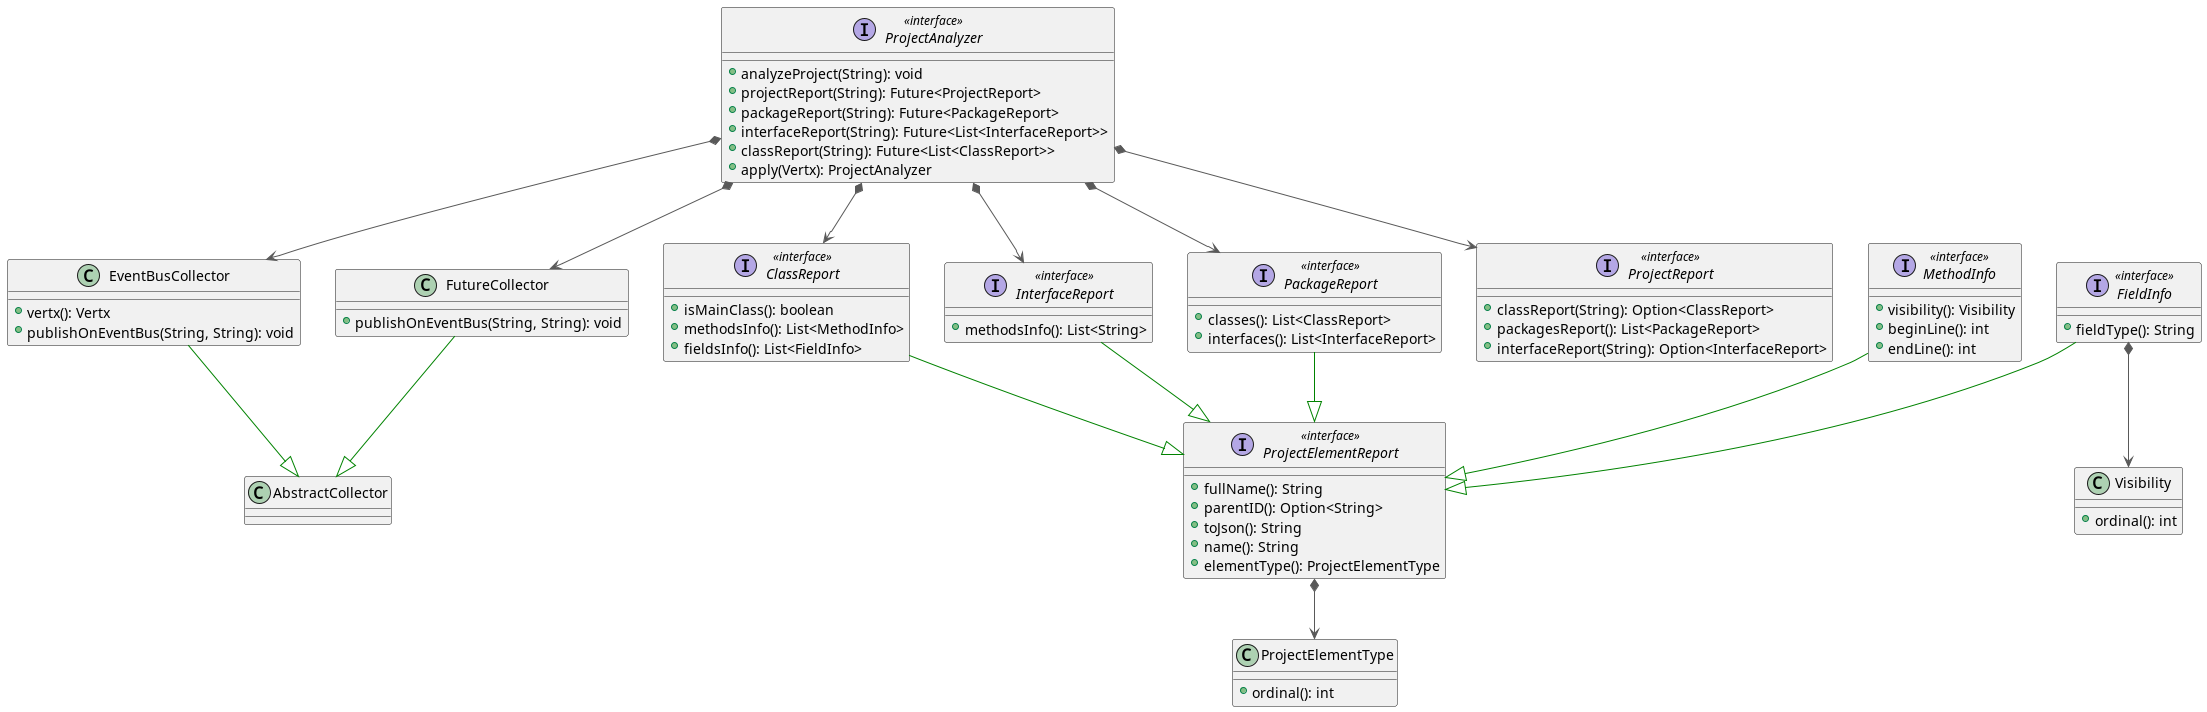
\includegraphics[angle=90, height=\textheight]{figures/EDAPProjectAnalyzer-0.png}
	\caption{Event Driven Asynchronous Programming: Project Analyzer.}
	\label{fig:edappa}
\end{figure}
\begin{figure}
	\centering
	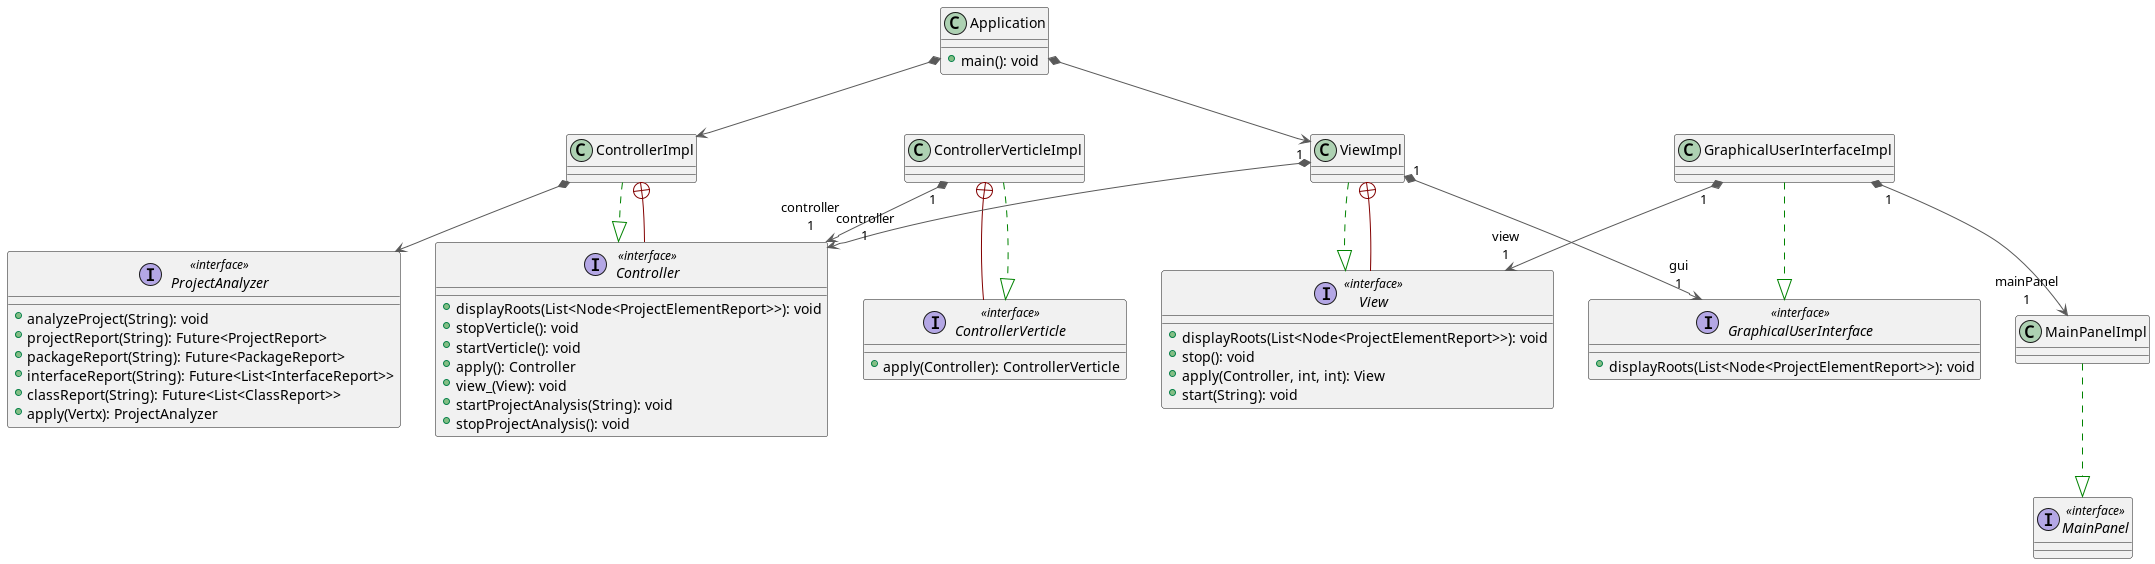
\includegraphics[angle=90, height=\textheight]{figures/EDAPMVC-0.png}
	\caption{Event Driven Asynchronous Programming: Model-View-Controller.}
	\label{fig:edapmvc}
\end{figure}
\begin{figure}
	\centering
	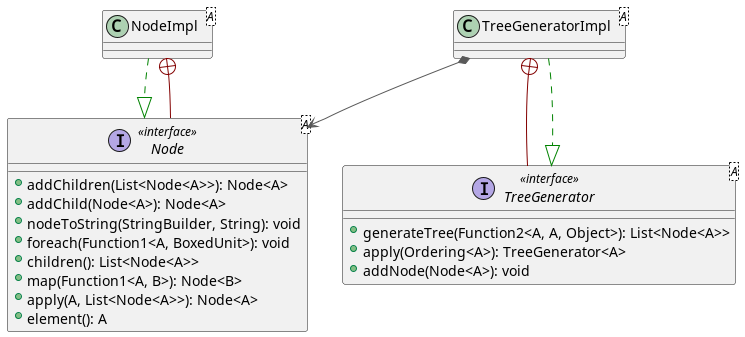
\includegraphics[width=\textwidth]{figures/TreeAlgorithm-0.png}
	\caption{Event Driven Asynchronous Programming: Tree Algorithm.}
	\label{fig:edapta}
\end{figure}
\begin{figure}[H]
	\centering
	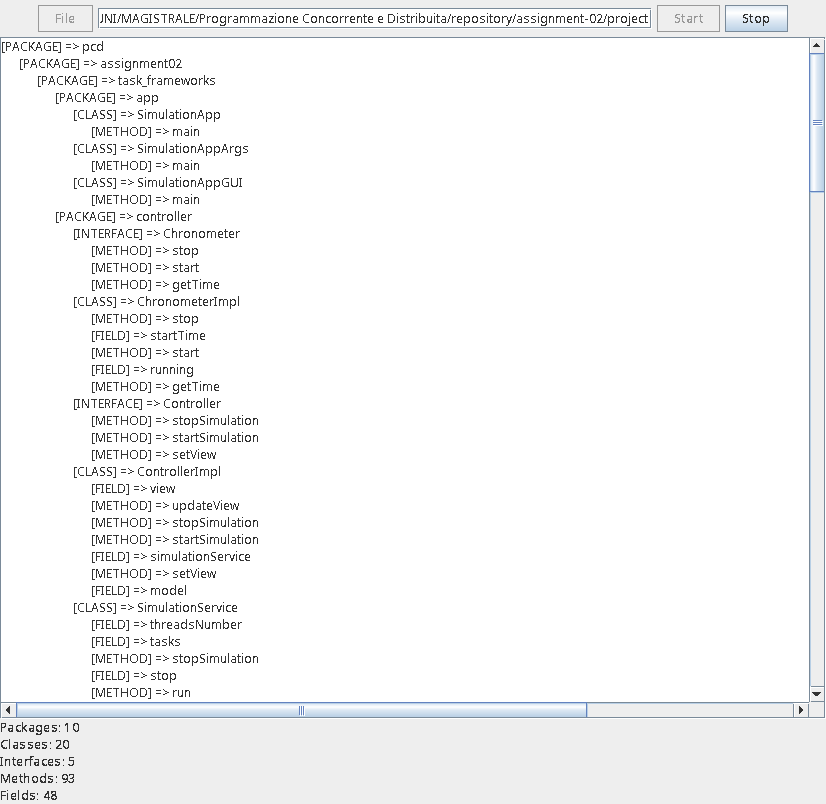
\includegraphics[width=\textwidth]{figures/project-analyzer-gui.png}
	\caption{Event Driven Asynchronous Programming: Interfaccia grafica}
	\label{fig:edapgui}
\end{figure}
%----------------------------------------------------------------------------------------
\chapter{Descrizione del Comportamento del Sistema} % possible chapter for Projects
\label{chap:Descrizione del Comportamento del Sistema}
%----------------------------------------------------------------------------------------
\section{Task Frameworks}
Nei Listati \ref{lst:UpdateSpeedTask}, \ref{lst:UpdatePositionTask} e \ref{lst:simulation_manager} viene mostrato il comportamento dei task Update Speed, Update Position e del simulation manager, rispettivamente.

In Figura \ref{fig:petri-net_task-frameworks} viene riportato il comportamento generale del simulation manager utilizzando 
le reti di Petri.

\begin{enumerate}

    \item Inizialmente il simulation manager avvia l'esecuzione dei task per l'aggiornamento della velocità dei corpi (istruzione: R0)
    \item I task eseguono l'aggiornamento della velocità dei corpi (istruzione: PS,QS 0)
    \item Il simulation manager rimane in attesa del completamento dell'esecuzione di tutti i task (istruzione: R1) prima di avviare l'esecuzione dei task per l'aggiornamento della posizione dei corpi (istruzione: R2)
    \item I task aggiornano le posizioni dei corpi e verificano le collisioni (istruzioni: PP,QP 0 e 1) 
    \item Il simulation manager rimane in attesa del completamento dell'esecuzione di tutti i task (istruzione: R3) prima di aggiornare la view e incrementare il numero di iterazione corrente (istruzioni: R4 e R5)

\newpage

\end{enumerate}

\begin{lstlisting}[label=lst:UpdateSpeedTask,caption=Pseudocodice di UpdateSpeedTask]
(PS,QS)0:		update bodies speed
\end{lstlisting}

\begin{lstlisting}[label=lst:UpdatePositionTask,caption=Pseudocodice di UpdatePositionTask]
(PP,QP)0:		update bodies position
(PP,QP)1:		check collisions
\end{lstlisting}

\begin{lstlisting}[label=lst:simulation_manager,caption=Pseudocodice del simulation manager]
		while(iteration < iterations && !stop):
R0:			executor.invokeAll(UpdateSpeedTasks)
R1:			wait all tasks to complete
R2:			executor.invokeAll(UpdatePositionTasks)
R3:			wait all tasks to complete
R4:     update the view
R5:     increment iteration
\end{lstlisting}

\begin{figure}[H]
	\centering
	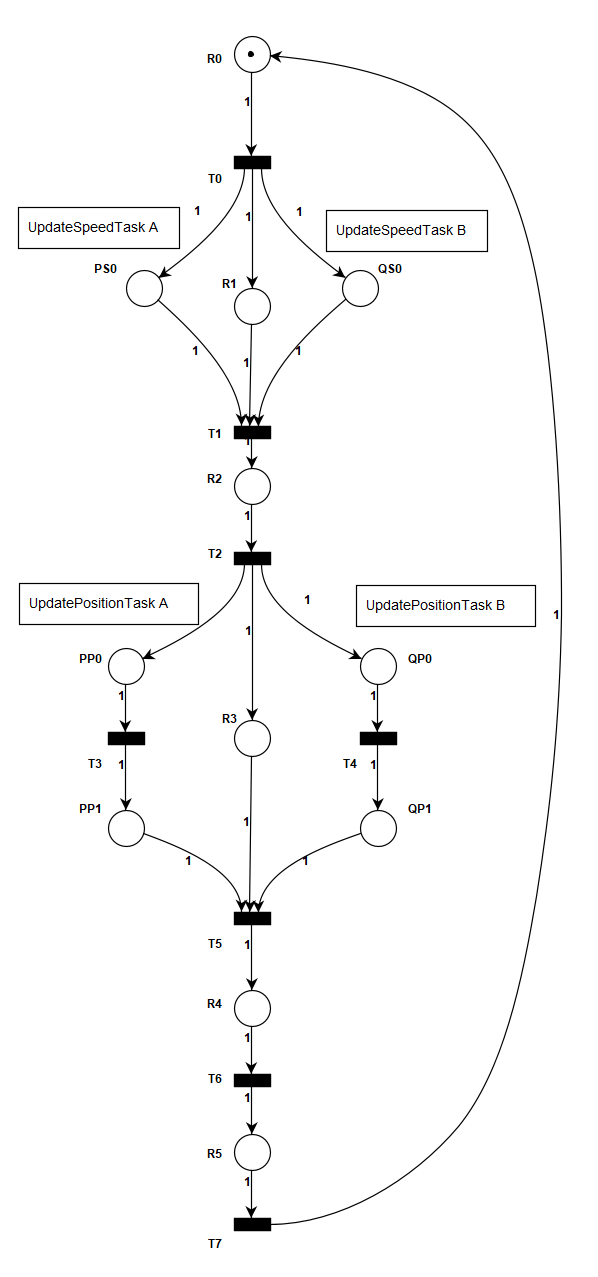
\includegraphics[width=0.7\linewidth]{figures/petri-net_task-frameworks.png}
	\caption{Task Frameworks: Rete di Petri}
	\label{fig:petri-net_task-frameworks}
\end{figure}


\section{Event Driven Asynchronous Programming e Reactive Programming}

Nel listato \ref{lst:projectReport} viene riportato il comportamento del metodo per la creazione del report di un progetto. Il relativo diagramma di Petri è rappresentato in Figura \ref{fig:petri-net_project-report}, prendendo come esempio un progetto con due package e due file per ogni package.
In primis, il file system viene analizzato ricorsivamente a partire dalla directory fornita per trovare tutti i package (istruzione: R0), successivamente viene effettuata l'analisi di ognuno dei package per trovare le classi e le interfacce al suo interno (istruzioni: PA,PB 0), le quali vengono a loro volta analizzate (istruzioni: FA,FB,FC,FD 0). Al completamento dell'analisi di tutti i file viene creato un \texttt{PackageReport} (istruzioni: PA,PB 1) e al termine dell'analisi di tutti i package viene generato un \texttt{ProjectReport} (istruzione: R1)

\begin{lstlisting}[label=lst:projectReport,caption=Pseudocodice della creazione del Report di un progetto]
(R)0:           analyze file system to get all packages
(PA,PB)0:       analyze package to get all files
(FA,FB,FC,FD)0: analyze file
(PA,PB)1:       wait all files to finish the analysis
(R)1:           create the project report object
\end{lstlisting}

\begin{figure}[H]
	\centering
	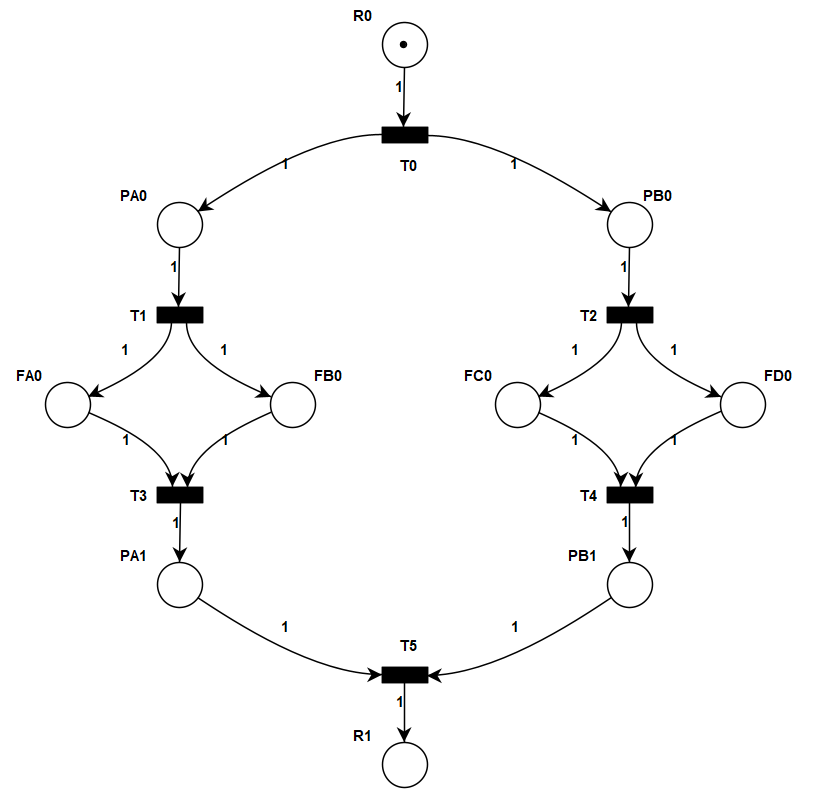
\includegraphics[width=1\linewidth]{figures/assignment-02_project-report_petri-net.png}
	\caption{Report di un progetto: Rete di Petri}
	\label{fig:petri-net_project-report}
\end{figure}
%----------------------------------------------------------------------------------------
\chapter{Verifica delle Prestazioni} % possible chapter for Projects
\label{chap:Verifica delle Prestazioni}
%----------------------------------------------------------------------------------------
La macchina su cui sono stati effettuati i test ha le seguenti caratteristiche:
\begin{itemize}
	\item Sistema operativo: Fedora 36 (GNU/Linux)
	\item Desktop environment: i3wm
	\item Versione kernel Linux: 5.17.7
	\item Memoria: 16GB, 3200Mhz
	\item CPU: AMD Ryzen 7 5700U
\end{itemize}
Descrizione dettagliata del processore:
\begin{itemize}
	\item Core: 8
	\item Thread: 16
	\item Clock base: 1.8GHz
	\item Clock max: 4.3GHz
	\item Cache L2: 4MB
	\item Cache L3: 8MB
\end{itemize}

Nelle tabelle \ref{tab:table1} e \ref{tab:table2} vengono riportati i risultati dei test effettuati usando Java Executor e Monitor, rispettivamente.
Quasi in tutti i casi la soluzione che fa uso degli Executor fornisce prestazioni migliori dell'implementazione con i Monitor.

\begin{table}[h!]
	\centering
	\begin{tabular}{ |c|c|c|c|c|c| } 
		\hline
		Numero test & Corpi & Iterazioni & Thread & Tempo esecuzione (ms) & Speedup \\
		\hline
0 & 100 & 1000 & 1 & 175 & 1.0 \\ 
 \hline
1 & 100 & 1000 & 9 & 146 & 1.2 \\ 
 \hline
2 & 100 & 1000 & 17 & 173 & 1.01 \\ 
 \hline
3 & 100 & 1000 & 99 & 299 & 0.59 \\ 
 \hline
4 & 100 & 10000 & 1 & 1036 & 1.0 \\ 
 \hline
5 & 100 & 10000 & 9 & 797 & 1.3 \\ 
 \hline
6 & 100 & 10000 & 17 & 1891 & 0.55 \\ 
 \hline
7 & 100 & 10000 & 99 & 3079 & 0.34 \\ 
 \hline
8 & 100 & 50000 & 1 & 4666 & 1.0 \\ 
 \hline
9 & 100 & 50000 & 9 & 3397 & 1.37 \\ 
 \hline
10 & 100 & 50000 & 17 & 9795 & 0.48 \\ 
 \hline
11 & 100 & 50000 & 99 & 15105 & 0.31 \\ 
 \hline
12 & 1000 & 1000 & 1 & 6967 & 1.0 \\ 
 \hline
13 & 1000 & 1000 & 9 & 3881 & 1.8 \\ 
 \hline
14 & 1000 & 1000 & 17 & 4114 & 1.69 \\ 
 \hline
15 & 1000 & 1000 & 99 & 4270 & 1.63 \\ 
 \hline
16 & 1000 & 10000 & 1 & 69620 & 1.0 \\ 
 \hline
17 & 1000 & 10000 & 9 & 37567 & 1.85 \\ 
 \hline
18 & 1000 & 10000 & 17 & 39891 & 1.75 \\ 
 \hline
19 & 1000 & 10000 & 99 & 41563 & 1.68 \\ 
 \hline
20 & 1000 & 50000 & 1 & 338323 & 1.0 \\ 
 \hline
21 & 1000 & 50000 & 9 & 193957 & 1.74 \\ 
 \hline
22 & 1000 & 50000 & 17 & 204168 & 1.66 \\ 
 \hline
23 & 1000 & 50000 & 99 & 208487 & 1.62 \\ 
 \hline
24 & 5000 & 1000 & 1 & 188145 & 1.0 \\ 
 \hline
25 & 5000 & 1000 & 9 & 98817 & 1.9 \\ 
 \hline
26 & 5000 & 1000 & 17 & 99086 & 1.9 \\ 
 \hline
27 & 5000 & 1000 & 99 & 98884 & 1.9 \\ 
 \hline
28 & 5000 & 10000 & 1 & 1860863 & 1.0 \\ 
 \hline
29 & 5000 & 10000 & 9 & 1022165 & 1.82 \\ 
 \hline
30 & 5000 & 10000 & 17 & 984490 & 1.89 \\ 
 \hline
31 & 5000 & 10000 & 99 & 989033 & 1.88 \\ 
 \hline
32 & 5000 & 50000 & 1 & 9105278 & 1.0 \\ 
 \hline
33 & 5000 & 50000 & 9 & 5171468 & 1.76 \\ 
 \hline
34 & 5000 & 50000 & 17 & 4985576 & 1.83 \\ 
 \hline
35 & 5000 & 50000 & 99 & 5025747 & 1.81 \\ 
 \hline
	\end{tabular}
	\caption{Risultati dei test con Java Executor}
	\label{tab:table1}
\end{table}

\begin{table}[h!]
	\centering
	\begin{tabular}{ |c|c|c|c|c|c| } 
		\hline
		Numero test & Corpi & Iterazioni & Thread & Tempo esecuzione (ms) & Speedup \\
		\hline
		0 & 100 & 1000 & 1 & 140 & 1.0 \\ 
 \hline
1 & 100 & 1000 & 9 & 177 & 0.79 \\ 
 \hline
2 & 100 & 1000 & 17 & 577 & 0.24 \\ 
 \hline
3 & 100 & 1000 & 99 & 3554 & 0.04 \\ 
 \hline
4 & 100 & 10000 & 1 & 980 & 1.0 \\ 
 \hline
5 & 100 & 10000 & 9 & 3439 & 0.28 \\ 
 \hline
6 & 100 & 10000 & 17 & 6503 & 0.15 \\ 
 \hline
7 & 100 & 10000 & 99 & 35622 & 0.03 \\ 
 \hline
8 & 100 & 50000 & 1 & 4442 & 1.0 \\ 
 \hline
9 & 100 & 50000 & 9 & 15854 & 0.28 \\ 
 \hline
10 & 100 & 50000 & 17 & 27406 & 0.16 \\ 
 \hline
11 & 100 & 50000 & 99 & 174241 & 0.03 \\ 
 \hline
12 & 1000 & 1000 & 1 & 6921 & 1.0 \\ 
 \hline
13 & 1000 & 1000 & 9 & 4082 & 1.7 \\ 
 \hline
14 & 1000 & 1000 & 17 & 4580 & 1.51 \\ 
 \hline
15 & 1000 & 1000 & 99 & 5212 & 1.33 \\ 
 \hline
16 & 1000 & 10000 & 1 & 69693 & 1.0 \\ 
 \hline
17 & 1000 & 10000 & 9 & 40159 & 1.74 \\ 
 \hline
18 & 1000 & 10000 & 17 & 45503 & 1.53 \\ 
 \hline
19 & 1000 & 10000 & 99 & 52843 & 1.32 \\ 
 \hline
20 & 1000 & 50000 & 1 & 339157 & 1.0 \\ 
 \hline
21 & 1000 & 50000 & 9 & 208154 & 1.63 \\ 
 \hline
22 & 1000 & 50000 & 17 & 233346 & 1.45 \\ 
 \hline
23 & 1000 & 50000 & 99 & 271759 & 1.25 \\ 
 \hline
24 & 5000 & 1000 & 1 & 181337 & 1.0 \\ 
 \hline
25 & 5000 & 1000 & 9 & 98946 & 1.83 \\ 
 \hline
26 & 5000 & 1000 & 17 & 99104 & 1.83 \\ 
 \hline
27 & 5000 & 1000 & 99 & 103171 & 1.76 \\ 
 \hline
28 & 5000 & 10000 & 1 & 1831471 & 1.0 \\ 
 \hline
29 & 5000 & 10000 & 9 & 1014055 & 1.81 \\ 
 \hline
30 & 5000 & 10000 & 17 & 984282 & 1.86 \\ 
 \hline
31 & 5000 & 10000 & 99 & 1051596 & 1.74 \\ 
 \hline
32 & 5000 & 50000 & 1 & 9167567 & 1.0 \\ 
 \hline
33 & 5000 & 50000 & 9 & 5060615 & 1.81 \\ 
 \hline
34 & 5000 & 50000 & 17 & 4992481 & 1.84 \\ 
 \hline
35 & 5000 & 50000 & 99 & 5230257 & 1.75 \\ 
 \hline
	\end{tabular}
	\caption{Risultati dei test con Monitor}
	\label{tab:table2}
\end{table}

\end{document}